\chapter{Grundlagen}
\label{sec:grundlagen}

\section{Grid Fins als Steuerelement von Flugkörpern im Hyperschall}
\subsection{Aufbau}
In der simpelsten Konfiguration bestehen Grid Fins aus einem äußeren Rahmen, der die innere Struktur von sich kreuzenden planaren Flächen stützt. Dieser einfache Aufbau gewährt hohe Stabilität bei vergleichsweise geringem Gewicht \cite{zellform} und lässt sich mittels 5 Parameter, wie in Abbildung \ref{abb_parameter} zu sehen, beschreiben. Die Wanddicke $d$ kann sich für den Rahmen ($d_R$) von der für das Gitter ($d_G$) unterscheiden. Aber auch innerhalb dieser Einteilung kann der Wert variieren, so ist häufig die Wandstärke in der Nähe der Einspannung zu erhöhen, um die dort auftretenden höheren Beanspruchungen zu ertragen. Ein umrahmtes Segment des Gitters wird als Zelle bezeichnet und ihre Dimension kann mit die Zellgröße $g$ beschrieben werden. Die Ausmaße der Grid Fins wird maßgeblich durch die Spannweite $b$ und die Höhe $h$ bestimmt. Die Querschnittsfläche $A$ steht in der Ausgangsstellung senkrecht zur Anströmung und wird vom Rahmen begrenzt. Normal zu dieser Fläche steht die Sehne mit einer im Vergleich zur planaren Finne deutlich kürzeren Länge $s$.\\
\begin{figure}[h]
	\centering
	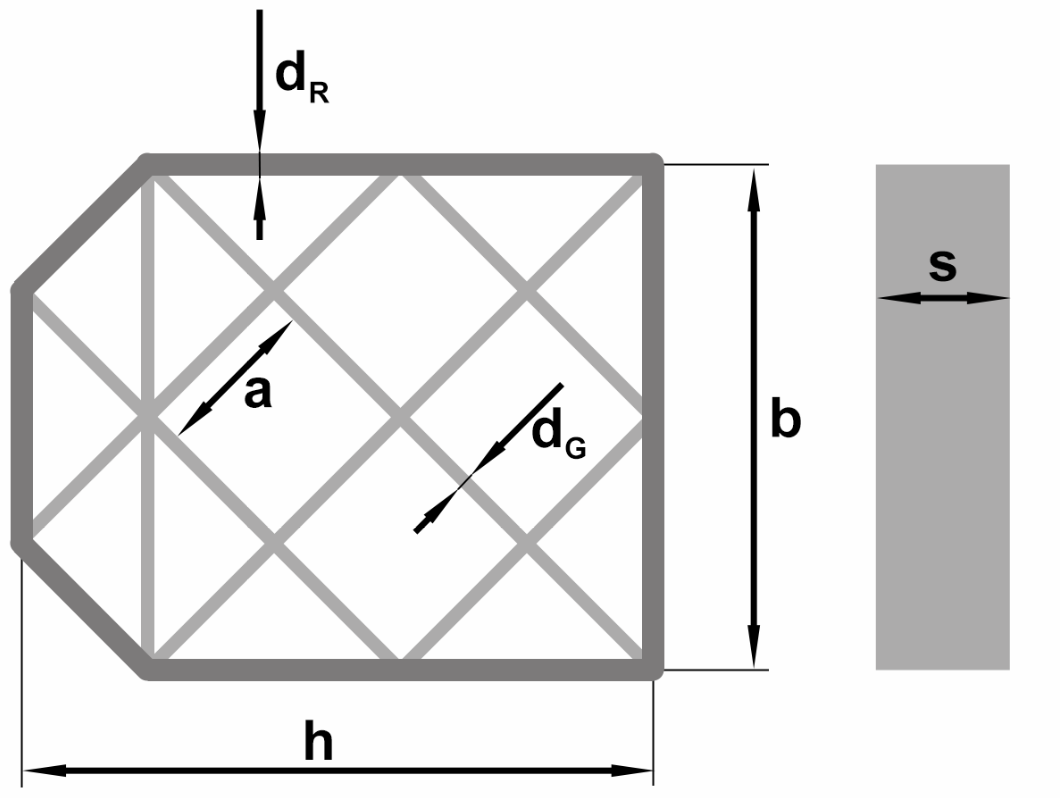
\includegraphics[width=0.6\textwidth]{Parameter.png}
	\caption{Aufbau eines einfachen Grid Fins}
	\label{abb_parameter}
\end{figure}\\
Grid Fins müssen nicht starr an einem Körper befestigt werden, sondern können um mehrere Achsen drehbar sein. Um sie für den Transport kompakt zu lagern, lassen sie sich an den Körper anlegen. Der Klappwinkel $\Lambda$ beschreibt den Ausschlag um eine den Körper an der Anbringung tangierende Achse. Ein Klappwinkel von $0^\circ$ entspricht hierbei den normalen in den Strömung ragenden Zustand und $90^\circ$ den eingeklappten. Zur Steuerung lassen sich die Grid Fins um eine Achse, die senkrecht aus dem Körper durch die Mitte des Grid Fins zeigt, verstellen. Ein Steuerwinkel von $\eta = 0^\circ$ ist auch hier wieder die Ausgangsstellung, die Sehne ist parallel zur Strömung. Bei $\eta = 90^\circ$ würde also die Seitenkante zur Anströmung zeigen, die Querschnittsfläche $A$, also das Gitter, wird nicht durchströmt.\\
\begin{figure}[h]
	\centering
	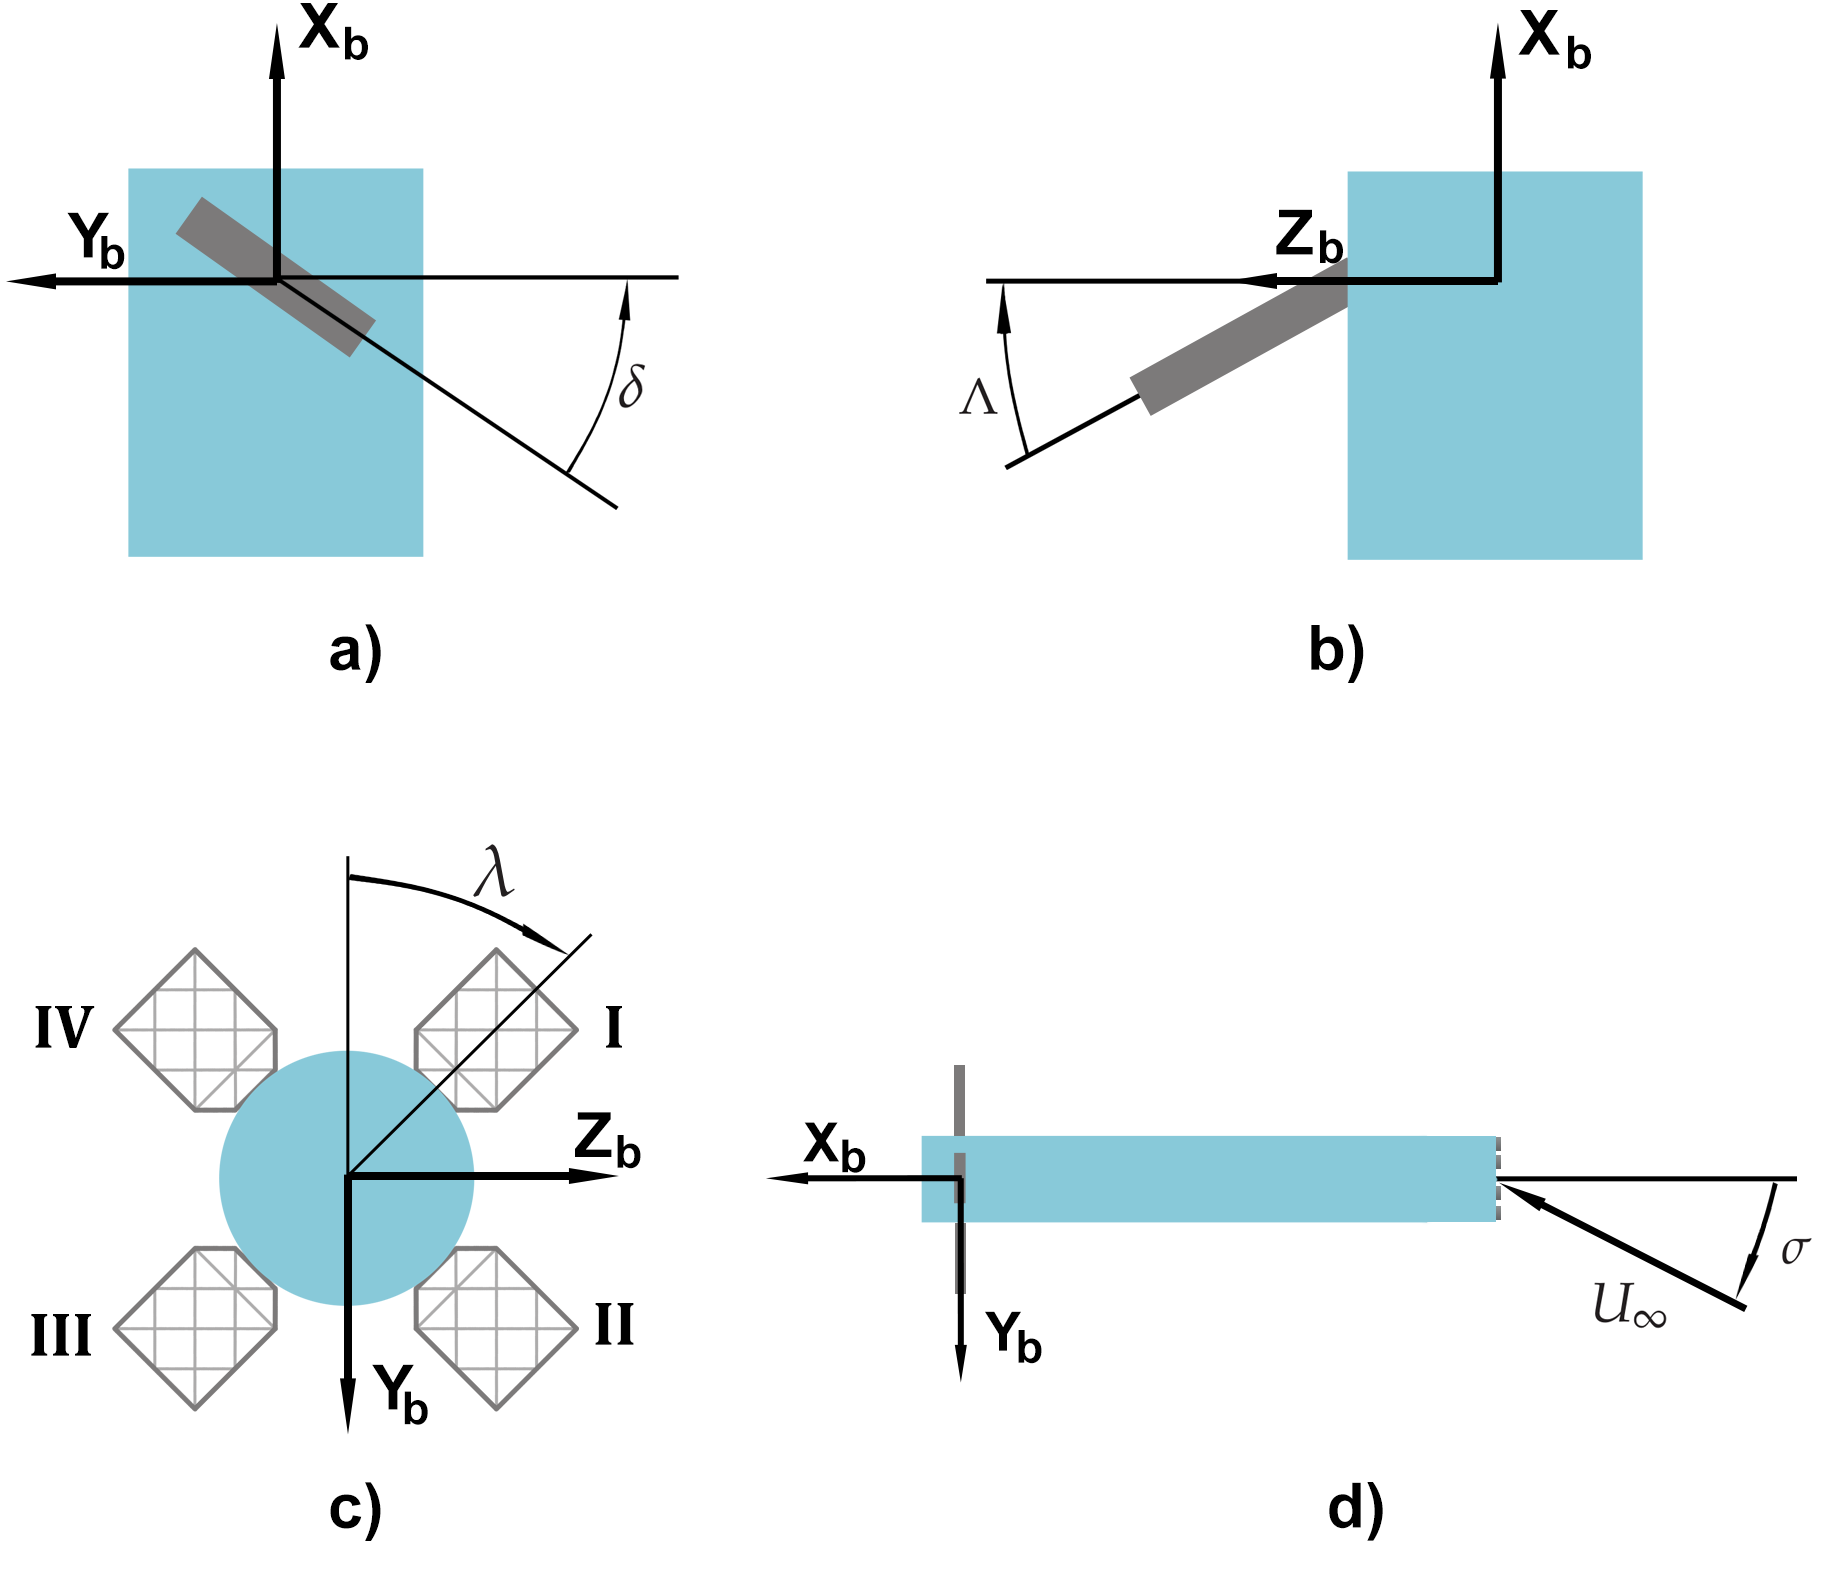
\includegraphics[width=0.8\textwidth]{Winkel.png}
	\caption{Winkel zur Beschreibung der Orientierung der Grid Fins zum Körper\\a) Steuerwinkel, b) Klappwinkel, c) Drehwinkel, d) Neigungswinkel des Körpers zur Anströmung}
	\label{abb_winkel}
\end{figure}\\
Um die Aerodynamik zu untersuchen reichen diese Winkel nicht aus, da die Anströmung nicht parallel zur Rakete liegen muss. Der Neigungswinkel des gesamten Moduls zur Antrömung $\sigma$ setzt sich unter realen Bedingungen aus dem Schiebewinkel und dem Bahnneigungswinkel, unter Vernachlässigung des Windes, zusammen. Für die in dieser Arbeit durchgeführten Untersuchungen ist eine solche Aufteilung aber irrelevant. Damit aber keine Informationen und somit Genauigkeit verloren geht, wird stattdessen die Orientierung der Grid Fins auf dem Umfang betrachtet. Verwendet wird hier eine Anordnung von vier gleichmäßig verteilten Steuerelementen. Das Koordinatensystem ist so definiert, dass es seinen Ursprung genau in der Mitte dieser Konfiguration hat und die positive X-Achse zur Spitze des Flugkörpers, also entgegen der Anströmung, zeigt. Bei $\sigma \neq 0$ zeigt auch die Y-Achse einem Anteil der Strömung entgegen. Die Z-Achse ist folglich nach den Rechtssystem orthogonal zu den anderen beiden ausgerichtet. Um nun die Orientierung der Grid Fins um die X-Achse herum beschreiben zu können wird der Rollwinkel $\lambda$ eingeführt. Wenn eine '+'-Konfiguration vorliegt, befinden sich die einzelnen Finnen auf den Koordinatenachsen (X, Y) und der Rollwinkel ist gleich null. Im Gegensatz dazu bei der 'x'-Konfiguration sind sie um einen Winkel von $\lambda = 45^\circ$ verdreht. Der Anstellwinkel $\alpha$, den ein einzelner Grid Fin erfährt, lässt sich aus dem Anstellwinkel des Körpers und, in Abhängigkeit vom Rollwinkel und welcher der Finnen überhaupt betrachtet wird, aus dem Klapp- und Steuerwinkel bestimmen.
\subsection{Strömung durch Grid Fins}
Bei niedrigen Strömungsgeschwindigkeiten im Unterschall haben Grid Fins auf Grund ihrer geringen Dicke keinen großen Einfluss auf das Fluid, welches nahezu ungestört durch das Gitter fließen kann \cite{sb-sharp}. Mit steigenden Machzahlen tritt aber zunehmend der Effekt auf, dass die Strömung um die stumpfe Vorderkante des Gitters in die Zelle hinein expandiert. Zusammen mit der Grenzschichtbildung an den Zellwänden, die effektiv zu Verengung der durchströmten Fläche führt, wir die Strömung innerhalb der Zellen auf Geschwindigkeiten beschleunigt, die über der der Anströmung liegen \cite{synopsis}.
%Bild aus synopsis

Der transsonische Bereich wird ab einer Anströmungsmachzahl von circa $Ma_\infty=0,8$ erreicht \cite{machgrenzen} und ist für die Aerodynamik der Grid Fins eine sehr kritische Problematik. Sobald die Strömung innerhalb des Gitters eine Machzahl von $1$ überschreitet, kommt es zu einem Verdichtungsstoß am Ausgang der Zellen, der mit steigender Machzahl an Stärke zunimmt. Dieser führt zu einer Drosselung der Strömung, was den Effekt hat, dass ein Teil der Strömung verdrängt wird und sich stattdessen um den Grid Fin herum bewegt. Steigt nun auch $Ma_\infty$ über $1$ löst sich der Stoß von den Gitterwänden und verbindet sich zu einer unregelmäßigen 3D-Struktur in der Abströmung \cite{stroemung}. Wächst $Ma_\infty$ weiter an, so kommt es zu einem Verdichtungsstoß vor dem Grid Fin. Dies führt dazu, dass innerhalb der Zellen keine Drosselung mehr vorliegt \cite{stroemung}, stattdessen wird die Strömung schon durch den Stoß vor dem Gitter um dieses herum verdrängt \cite{synopsis}. Von den Vorderkanten gehen Schockwellen aus, die auf die benachbarten Wände treffen und mit ihnen interagieren \cite{synopsis}. Steigt die Machzahl weiter an, so befinden sich diese Wellen auf steileren Bahnen bis sie gar nicht mehr auf die anderen Wände treffen. Des weiteren nähert sich der Verdichtungsstoß vor dem Grid Fin diesem immer weiter mit größer werdenden Strömungsgeschwindigkeiten an, bis es abgesehen von der direkten Umgebung der Wände gar nicht mehr zum Stoß kommt. Die einzelnen Zellen fungieren nun als Überschalldüse \cite{stroemung}, sodass die Strömung in den meisten Bereichen nicht mehr auf den Unterschall abgebremst wird. Der Stoß wurde vom Gitter "verschluckt".

Als ein besonderer Bereich ist noch die Ansatzregion zu betrachten, in der der Grid Fin an der Rakete angebracht ist. Schnittstellen von Wänden stellen ein erhöhtes Potenzial für blockierte Strömung dar. In der Ansatzregion befinden sich nicht nur vielen von diesen Schnittstellen, sondern auch die Dicke ist hier meistens am größten. Dies in Kombination mit einer schon durch die Grenzschichtwirkung des Körpers verzögerte Strömung, führt zu einer relativ großen Region verlangsamter Strömung oder gar Rückströmung, die mit der Machzahl an Größe gewinnt \cite{stroemung}. Bei einer Machzahl von ungefähr $Ma_\infty = 2$ erreicht diese jedoch ein Maximum, da die Strömung bei weiter steigenden Geschwindigkeiten von der umgebenden mitgerissen wird und diese Region somit wieder an Größe und Bedeutung verliert \cite{stroemung}.
\subsection{Aerodynamische Beiwerte und Vergleich zu planaren Finnen}
\subsection{Bisherige Implementierung/ Grid Fin Varianten}

\section{Wiedereintrittsbedingungen}

\section{Das Air-Launchsystem Valkyrie}

